\chapter{First Chapter}

\blindtext
\begin{equation}
	\p(x \given \mathcal{D}) = \frac{ \p(\mathcal{D} \given x) \p(x) }{ \p(\mathcal{D}) }
	\label{eq:Bayes}
\end{equation}
\blindtext

\section{Bayes vs.\ Frequentist}
\blindtext

\begin{figure}
	\centering
	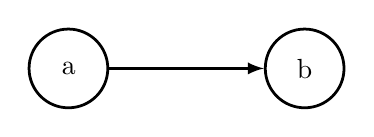
\begin{tikzpicture}
		\node (a) [draw, circle, minimum size=1cm, line width=1pt] {a};
		\node (b) [draw, circle, minimum size=1cm, line width=1pt] at (3,0) {b};
		\draw [-latex, line width=1pt] (a) -- (b);
	\end{tikzpicture}
	\caption{Graphical Model}
	\label{fig:GM}
\end{figure}

\blindtext

\section{Referencing Examples}
\cref{eq:Bayes} shows Bayes' theorem. \cref{fig:GM} depicts a graphical model. The Dirichlet process is discussed in \cite{ferguson1973bayesian}.